\documentclass[
    a4paper,
    twocolumn,
]{article}

% Table insertions
% --------------------------------------------------
\usepackage{graphics}

% Image insertions
% --------------------------------------------------
\usepackage{graphicx}
\usepackage[belowskip=-3pt,aboveskip=8pt]{caption}
\graphicspath{{./images/}}

% Input and font encoding
% --------------------------------------------------
\usepackage[utf8]{inputenc}
\usepackage[T1]{fontenc}

% biblatex --- Bibliography setup
% --------------------------------------------------
\usepackage[
    backend=biber,
    style=numeric,
    sorting=none,
]{biblatex}

\addbibresource{sources.bib}

% hyperref --- Hyperlinks in PDF
% --------------------------------------------------
\usepackage[pdfusetitle]{hyperref}

% Set colors of links
\hypersetup{
    colorlinks=true,
    linkcolor=magenta,
    citecolor=,
    urlcolor=blue,
}

% Allow line-breaks in links and URLs
\hypersetup{breaklinks=true}

% Use the normal document font for URLs rather than monospace
\urlstyle{same}

% Document Metadata
% --------------------------------------------------
\title{INF3200: Mandatory Assignment 1}
\author{Yasiru Rathsara Witharanage}
\date{\today}

% Document
% --------------------------------------------------
\begin{document}

\maketitle

\begin{abstract}
    In an ever-growing tech-world, the necessity of storing and accessing data is vital. With the expansion of industry and users, data-stores are being required to address additional features apart from its main objective, such as scalability, replication, accessibility etc. To this end, distributed data-stores have been more useful and applicable. In this study, I have implemented a distributed hash table using chord~\cite{1} and conducted few experiments to observe how its performance differs with cluster's scale.
\end{abstract}

\section{Introduction}

The primary objective of this study is to build a system of distributed nodes acting as a single key-value store with the assistance of a distributed hash table 'chord', which uses a ring network of individual nodes with distributed memory each with the knowledge of only a partition of the entire network. This store exposes the following HTTP endpoints for querying and debugging purposes.

\begin{itemize}
	\item PUT /storage/key - to store a value provided in the raw body
	\item GET /storage/key - to retrieve the value of a key (returned in raw body)
	\item GET /neighbors - to retrieve the neighbours of a node
\end{itemize}

\section{Project Description}
\subsection{Design}

Each individual node in the network is given an id based on the SHA256 hash value of its own hostname. Thus, specific instances were chosen to resemble and organize the ring structure such that there are no multiple instances for the same id. Fig.1 shows one of such structures with 16 nodes used in the experiments of this study along with generated node ids and hostnames.

\setlength{\intextsep}{10pt plus 2pt minus 2pt}
\begin{figure}[!ht]
	\centering
	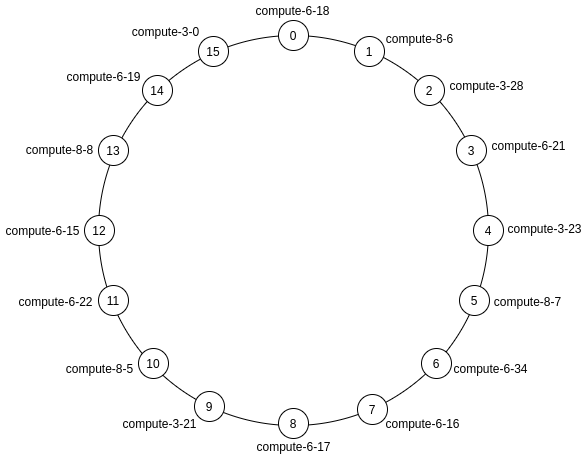
\includegraphics[width=7.5cm]{16-structure.png}
	\caption{Ring structure with 16-nodes}
\end{figure}

Each node is only aware of its neighbours, i.e. predecessor and successor. These values can be configured before the execution of a node. \\

Whenever a query is received by a node, it initially checks whether the requested key belongs to itself and if not, it proceeds to the immediate successor. This process is iterated until the correct node for key is discovered and the corresponding response is returned along the same route. 

\subsection{Implementation}

Golang was used for the implementation of chord with a flat-hierarchical code structure and different layers for each functionality. HTTP endpoints listed previously were implemented in HTTP layer while node layer contains details (node id, predecessor, successor) related with the node along with validating key function. SHA256 was used for hashing of both key and node id to match with relevant buckets. A separate HTTP client was used in neighbour layer to proceed any request with a key that does not belong to the corresponding node. All key-value entry pairs are stored in an in-memory map which is specifically designed for concurrent use.\\

A sample set is given below for the configuration values of parameters required by the implementation but however user is allowed to provide his own desired values for service configurations. Predecessor and successor ports can be given null if they are same as the port of current node.

\begin{verbatim}
	# service configs
	port: 52520
	max_num_of_nodes: 16
	request_timeout_sec: 2
	ttl_min: 180
	
	# neighbour configs
	finger_table_enabled: false
	neighbour_check: false
	predecessor: "compute-1-1"
	predecessor_port: ""
	successor: "compute-1-1"
	successor_port: ""
	
	# logger configs
	colors_enabled: true
	log_level: "TRACE"
	file_path: true
\end{verbatim}

\section{Evaluation}

Experiments were carried out to measure and evaluate latency variation under different circumstances. A separate client was implemented for this testing purpose and can be found under tester directory. \\

In these experiments, a number of requests was sent and total latency of the whole batch was measured in order to calculate the average latency per request in different scenarios. Each attempt was made 3 times and the resultant average total latency value was considered for the calculations. This entire process was done several times by changing load (number of requests) and number of nodes in the cluster. \\

A set of 15 dummy requests was used in these attempts where each request consists of a key belonging to a separate bucket. This set was iterated as many times as required until the number of requests being tested was matched.\\

Below shows the tables containing hardware specifications of nodes and sets of nodes used in each experiment.

\begin{table}[!ht]
\centering
\resizebox{\columnwidth}{!}{%
\begin{tabular}{|c | c | c | c | c | c|} 
	\hline
	Node ID & Hostname & Model & CPUs & Cores & Processors\\
	\hline
	0 & compute-6-18 & Lenovo P310 & 1 & 4 & 4 \\ 
	\hline
	1 & compute-8-6 & Lenovo m93p & 1 & 4 & 8 \\ 
	\hline
	2 & compute-3-28 & Dell T3600 & 1 & 4 & 4 \\ 
	\hline
	3 & compute-6-21 & Lenovo P310 & 1 & 4 & 4 \\ 
	\hline
	4 & compute-3-23 & Dell T3600 & 1 & 4 & 4 \\ 
	\hline
	5 & compute-8-7 & Lenovo m93p & 1 & 4 & 8 \\ 
	\hline
	6 & compute-6-34 & Lenovo P310 & 1 & 4 & 4 \\ 
	\hline
	7 & compute-6-16 & Lenovo P310 & 1 & 4 & 4 \\ 
	\hline
	8 & compute-6-17 & Lenovo P310 & 1 & 4 & 4 \\ 
	\hline
	9 & compute-3-21 & Dell T3600 & 1 & 4 & 4 \\ 
	\hline
	10 & compute-8-5 & Lenovo m93p & 1 & 4 & 8 \\ 
	\hline
	11 & compute-6-22 & Lenovo P310 & 1 & 4 & 4 \\ 
	\hline
	12 & compute-6-15 & Lenovo P310 & 1 & 4 & 4 \\ 
	\hline
	13 & compute-8-8 & Lenovo m93p & 1 & 4 & 8 \\ 
	\hline
	14 & compute-6-19 & Lenovo P310 & 1 & 4 & 4 \\ 
	\hline
	15 & compute-3-0 & Dell T3600 & 1 & 4 & 4 \\ 
	\hline
\end{tabular}%
}
\caption{Hardware specification of nodes}
\end{table}

\begin{table}[!ht]
	\centering
	\resizebox{\columnwidth}{!}{%
		\begin{tabular}{|c | l|} 
			\hline
			Number of nodes &\multicolumn{1}{|c|}{Node IDs} \\
			\hline
			1 & 10 \\ 
			\hline
			2 & 0, 7 \\
			\hline
			4 & 2, 5, 8, 11 \\
			\hline
			8 & 0, 1, 4, 6, 8, 9, 10, 13 \\
			\hline
			16 & 0, 1, 2, 3, 4, 5, 6, 7, 8, 9, 10, 11, 12, 13, 14, 15 \\
			\hline
		\end{tabular}%
	}
	\caption{Nodes used in each experiment}
\end{table}

\section{Results}

\begin{table}[!ht]
	\centering
	\resizebox{\columnwidth}{!}{%
		\begin{tabular}{|c | c | c | c|} 
			\hline
			Number of nodes & Size of load (No. of requests) & GET - Average time (ms) & PUT - Average time (ms) \\
			\hline
			& 16 &  &  \\
			\cline{2-4}
			1 & 100 & 0.09557974 & 0.0995189 \\
			\cline{2-4}
			& 1000 & 0.058 & 0.062 \\
			\hline
			& 16 & 0.345 & 0.3125 \\
			\cline{2-4}
			2 & 100 & 0.12 & 0.11 \\
			\cline{2-4}
			& 1000 & 0.065 & 0.064 \\
			\hline
			& 16 & & \\
			\cline{2-4}
			4 & 100 & & \\
			\cline{2-4}
			& 1000 & & \\
			\hline
			& 16 & 0.8958 & 0.9375 \\
			\cline{2-4}
			8 & 100 & 0.25 & 0.2667 \\
			\cline{2-4}
			& 500 & 0.158 & 0.144 \\
			\hline
			& 16 & 1.5208 & 1.5625 \\
			\cline{2-4}
			16 & 100 & 0.38 & 0.38 \\
			\cline{2-4}
			& 500 & 0.158 & 0.146\\
			\hline
		\end{tabular}%
	}
	\caption{Results of experiments}
\end{table}

\section{Discussion}
\section{Conclusion}

\printbibliography

\end{document}
